%==============================================================
%  Figura 8.19 - Arresto di un azionamento con convertitore di
%  frequenza comandato da PLC a seguito di un comando di arresto
%  di emergenza (Esempio 10)
%  Adattamento in italiano della Figura 8.19 dell'IFA Report 2/2017
%
%  I simboli riproducono quelli dell'originale: le coordinate sono
%  ricavate dal disegno di partenza (1 cm = 70 px, origine
%  nell'angolo in alto a sinistra della cornice). Nessun cambio di
%  corpo del font: le etichette sono ingrandite con "scale" (vedere
%  la nota nella Figura 8.3). Le etichette START e STOP restano in
%  inglese, come nella Figura 8.13.
%==============================================================
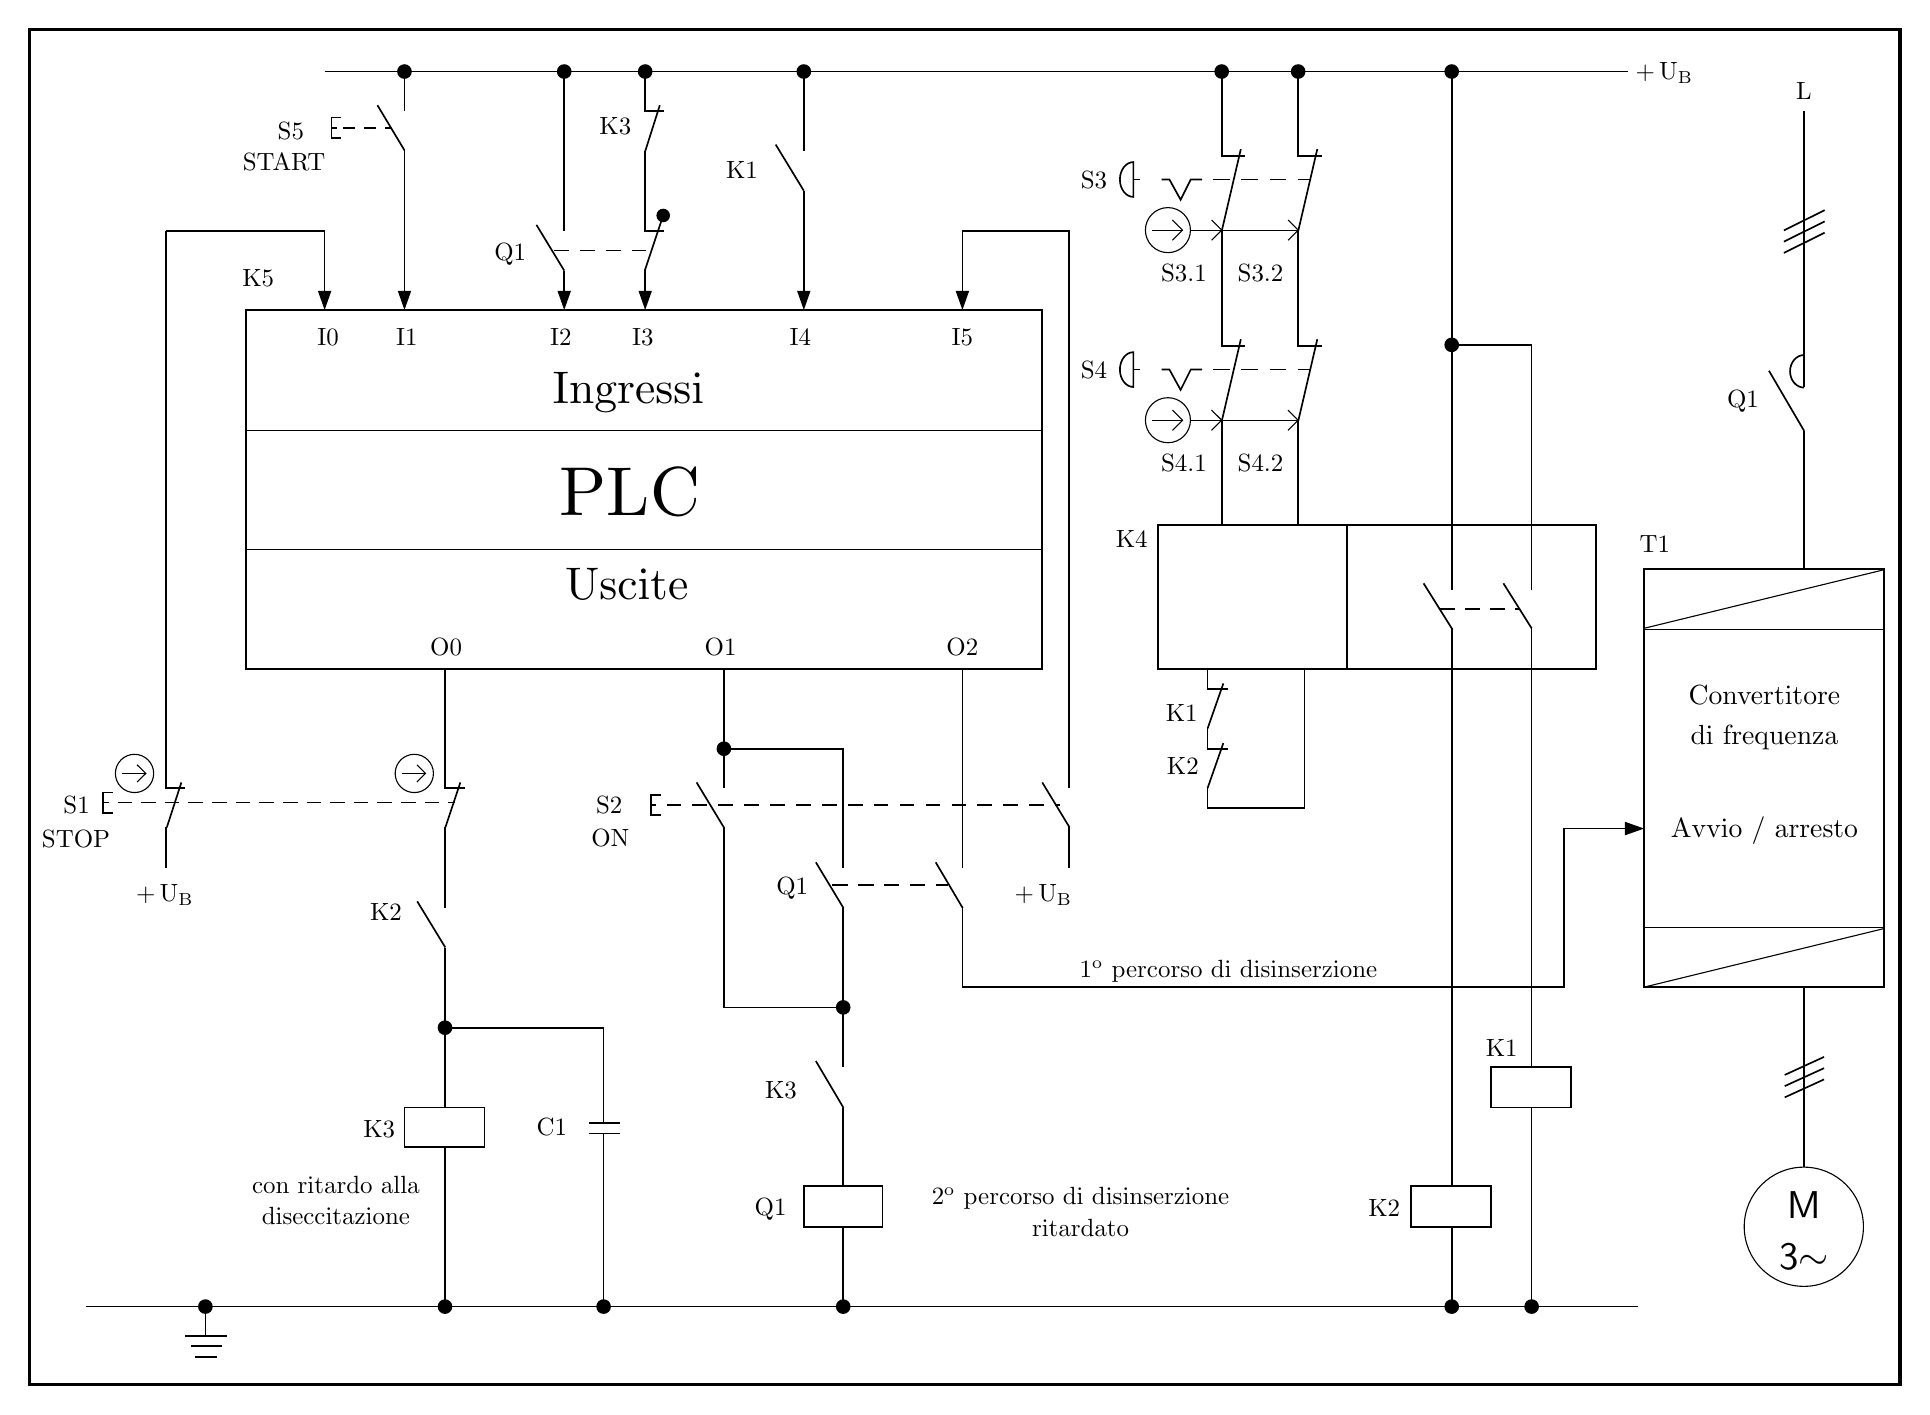
\begin{tikzpicture}[
  font=\normalsize,
  filo/.style={draw=black, line width=0.6pt},
  sottile/.style={draw=black, line width=0.4pt},
  meccanico/.style={draw=black, line width=0.6pt},
  etichetta/.style={inner sep=0pt, scale=0.9},
  testo/.style={inner sep=0pt, scale=1.0},
  medio/.style={inner sep=0pt, scale=1.65},
  grande/.style={inner sep=0pt, scale=2.5},
  motore/.style={inner sep=0pt, scale=1.4, font=\sffamily},
  nodo/.style={circle, fill=black, inner sep=0pt, minimum size=0.186cm}
]

%--------------------------------------------------------------
% Cornice
%--------------------------------------------------------------
\draw[draw=black, line width=1.2pt] (0.000,-0.000) rectangle (23.757,-17.214);

%--------------------------------------------------------------
% Linea di alimentazione +U_B
%--------------------------------------------------------------
\draw[filo] (3.750,-0.536) -- (20.307,-0.536);
\node[nodo] at (4.764,-0.536) {};
\node[nodo] at (6.793,-0.536) {};
\node[nodo] at (7.821,-0.536) {};
\node[nodo] at (9.836,-0.536) {};
\node[nodo] at (15.143,-0.536) {};
\node[nodo] at (16.114,-0.536) {};
\node[nodo] at (18.064,-0.536) {};
\node[etichetta, anchor=base west] at (20.393,-0.636) {+\,U\textsubscript{B}};

%--------------------------------------------------------------
% S5: pulsante di START (contatto di chiusura) -> I1
%--------------------------------------------------------------
\draw[filo] (4.764,-0.536) -- (4.764,-1.036);
\draw[filo] (4.421,-0.964) -- (4.764,-1.536);
\draw[filo] (4.764,-1.536) -- (4.764,-3.321);
\fill (4.679,-3.321) -- (4.850,-3.321) -- (4.764,-3.564) -- cycle;
\draw[filo] (3.964,-1.121) -- (3.836,-1.121) -- (3.836,-1.379) -- (3.964,-1.379);
\draw[filo] (3.836,-1.250) -- (3.907,-1.250);
\draw[meccanico, dash pattern=on 0.157cm off 0.114cm] (3.979,-1.250) -- (4.593,-1.250);
\node[etichetta, anchor=base] at (3.321,-1.393) {S5};
\node[etichetta, anchor=base] at (3.236,-1.793) {START};

%--------------------------------------------------------------
% K5 -> I0
%--------------------------------------------------------------
\draw[filo] (1.736,-2.564) -- (3.750,-2.564) -- (3.750,-3.321);
\fill (3.664,-3.321) -- (3.836,-3.321) -- (3.750,-3.564) -- cycle;
\node[etichetta, anchor=base] at (2.907,-3.264) {K5};

%--------------------------------------------------------------
% Q1: contatto ausiliario di chiusura -> I2
%--------------------------------------------------------------
\draw[filo] (6.793,-0.536) -- (6.793,-2.564);
\draw[filo] (6.440,-2.483) -- (6.793,-3.064);
\draw[filo] (6.793,-3.064) -- (6.793,-3.321);
\fill (6.707,-3.321) -- (6.879,-3.321) -- (6.793,-3.564) -- cycle;
\node[etichetta, anchor=base] at (6.107,-2.936) {Q1};

%--------------------------------------------------------------
% K3: contatto di apertura e Q1: contatto a specchio -> I3
%--------------------------------------------------------------
\draw[filo] (7.821,-0.536) -- (7.821,-1.036) -- (8.064,-1.036);
\draw[filo] (8.007,-0.964) -- (7.821,-1.550);
\draw[filo] (7.821,-1.550) -- (7.821,-2.564) -- (8.064,-2.564);
\fill (8.050,-2.364) circle (0.086);
\draw[filo] (8.050,-2.364) -- (7.821,-3.050);
\draw[filo] (7.821,-3.050) -- (7.821,-3.321);
\fill (7.736,-3.321) -- (7.907,-3.321) -- (7.821,-3.564) -- cycle;
\draw[meccanico, dash pattern=on 0.186cm off 0.143cm] (6.664,-2.807) -- (7.907,-2.807);
\node[etichetta, anchor=base] at (7.443,-1.336) {K3};

%--------------------------------------------------------------
% K1: contatto di chiusura -> I4
%--------------------------------------------------------------
\draw[filo] (9.836,-0.536) -- (9.836,-1.550);
\draw[filo] (9.479,-1.464) -- (9.836,-2.050);
\draw[filo] (9.836,-2.050) -- (9.836,-3.321);
\fill (9.750,-3.321) -- (9.921,-3.321) -- (9.836,-3.564) -- cycle;
\node[etichetta, anchor=base] at (9.050,-1.893) {K1};

%--------------------------------------------------------------
% S2: secondo contatto di chiusura -> I5
%--------------------------------------------------------------
\draw[filo] (13.207,-9.636) -- (13.207,-2.564) -- (11.850,-2.564) -- (11.850,-3.321);
\fill (11.764,-3.321) -- (11.936,-3.321) -- (11.850,-3.564) -- cycle;

%--------------------------------------------------------------
% PLC
%--------------------------------------------------------------
\draw[filo] (2.750,-3.564) rectangle (12.864,-8.121);
\draw[filo] (2.750,-5.093) -- (12.864,-5.093);
\draw[filo] (2.750,-6.607) -- (12.864,-6.607);
\node[etichetta, anchor=base] at (3.793,-4.021) {I0};
\node[etichetta, anchor=base] at (4.793,-4.021) {I1};
\node[etichetta, anchor=base] at (6.750,-4.021) {I2};
\node[etichetta, anchor=base] at (7.793,-4.021) {I3};
\node[etichetta, anchor=base] at (9.793,-4.021) {I4};
\node[etichetta, anchor=base] at (11.850,-4.021) {I5};
\node[medio, anchor=base] at (7.607,-4.750) {Ingressi};
\node[grande, anchor=base] at (7.629,-6.179) {PLC};
\node[medio, anchor=base] at (7.586,-7.236) {Uscite};
\node[etichetta, anchor=base] at (5.293,-7.950) {O0};
\node[etichetta, anchor=base] at (8.779,-7.950) {O1};
\node[etichetta, anchor=base] at (11.850,-7.950) {O2};

%--------------------------------------------------------------
% S1: pulsante di STOP (due contatti di apertura ad azionamento
% meccanico positivo)
%--------------------------------------------------------------
\draw[filo] (1.736,-2.564) -- (1.736,-9.636) -- (1.979,-9.636);
\draw[filo] (1.931,-9.564) -- (1.746,-10.136);
\draw[filo] (1.736,-10.136) -- (1.736,-10.650);
\draw[sottile] (1.336,-9.450) circle (0.243);
\draw[sottile] (1.179,-9.450) -- (1.479,-9.450);
\draw[sottile] (1.369,-9.341) -- (1.479,-9.450) -- (1.369,-9.559);
\node[etichetta, anchor=base] at (1.721,-11.079) {+\,U\textsubscript{B}};
\draw[filo] (5.279,-8.121) -- (5.279,-9.636) -- (5.536,-9.636);
\draw[filo] (5.474,-9.564) -- (5.283,-10.136);
\draw[filo] (5.279,-10.136) -- (5.279,-11.164);
\draw[sottile] (4.889,-9.450) circle (0.243);
\draw[sottile] (4.731,-9.450) -- (5.031,-9.450);
\draw[sottile] (4.922,-9.341) -- (5.031,-9.450) -- (4.922,-9.559);
\draw[filo] (1.064,-9.693) -- (0.936,-9.693) -- (0.936,-9.950) -- (1.064,-9.950);
\draw[filo] (0.936,-9.821) -- (1.007,-9.821);
\draw[meccanico, dash pattern=on 0.186cm off 0.114cm] (1.121,-9.821) -- (5.407,-9.821);
\node[etichetta, anchor=base] at (0.600,-9.964) {S1};
\node[etichetta, anchor=base] at (0.593,-10.393) {STOP};

%--------------------------------------------------------------
% O0: contatto di chiusura di K2, bobina di K3 con ritardo alla
% diseccitazione e condensatore C1
%--------------------------------------------------------------
\draw[filo] (4.926,-11.074) -- (5.283,-11.660);
\draw[filo] (5.279,-11.664) -- (5.279,-13.693);
\draw[filo] (4.764,-13.693) rectangle (5.779,-14.193);
\draw[filo] (5.279,-14.193) -- (5.279,-16.221);
\node[nodo] at (5.279,-12.679) {};
\draw[filo] (5.279,-12.679) -- (7.293,-12.679) -- (7.293,-13.893);
\draw[filo] (7.107,-13.893) -- (7.507,-13.893);
\draw[filo] (7.107,-14.021) -- (7.507,-14.021);
\draw[filo] (7.293,-14.021) -- (7.293,-16.221);
\node[etichetta, anchor=base] at (4.529,-11.321) {K2};
\node[etichetta, anchor=base] at (4.443,-14.079) {K3};
\node[etichetta, anchor=base] at (6.636,-14.050) {C1};
\node[etichetta, anchor=base] at (3.893,-14.779) {con ritardo alla};
\node[etichetta, anchor=base] at (3.893,-15.179) {diseccitazione};

%--------------------------------------------------------------
% O1: pulsante S2 (ON), contatto ausiliario di Q1 (automantenimento),
% contatto di chiusura di K3 e bobina di Q1
%--------------------------------------------------------------
\draw[filo] (8.821,-8.121) -- (8.821,-9.636);
\node[nodo] at (8.821,-9.136) {};
\draw[filo] (8.821,-9.136) -- (10.336,-9.136) -- (10.336,-10.650);
\draw[filo] (8.474,-9.564) -- (8.821,-10.136);
\draw[filo] (8.821,-10.136) -- (8.821,-12.421) -- (10.336,-12.421);
\node[nodo] at (10.336,-12.421) {};
\draw[filo] (8.021,-9.721) -- (7.893,-9.721) -- (7.893,-9.979) -- (8.021,-9.979);
\draw[filo] (7.893,-9.850) -- (7.964,-9.850);
\draw[meccanico, dash pattern=on 0.186cm off 0.143cm] (8.093,-9.850) -- (13.093,-9.850);
\draw[filo] (12.864,-9.564) -- (13.211,-10.136);
\draw[filo] (13.207,-10.136) -- (13.207,-10.650);
\node[etichetta, anchor=base] at (12.879,-11.079) {+\,U\textsubscript{B}};
\node[etichetta, anchor=base] at (7.364,-9.964) {S2};
\node[etichetta, anchor=base] at (7.379,-10.379) {ON};
\draw[filo] (9.989,-10.579) -- (10.340,-11.160);
\draw[filo] (10.336,-11.164) -- (10.336,-13.179);
\draw[filo] (9.989,-13.103) -- (10.340,-13.697);
\draw[filo] (10.336,-13.693) -- (10.336,-14.693);
\draw[filo] (9.836,-14.693) rectangle (10.836,-15.207);
\draw[filo] (10.336,-15.207) -- (10.336,-16.221);
\node[etichetta, anchor=base] at (9.689,-10.993) {Q1};
\node[etichetta, anchor=base] at (9.546,-13.579) {K3};
\node[etichetta, anchor=base] at (9.414,-15.064) {Q1};
\node[etichetta, anchor=base] at (13.350,-14.921) {2\textsuperscript{o} percorso di disinserzione};
\node[etichetta, anchor=base] at (13.350,-15.336) {ritardato};

%--------------------------------------------------------------
% O2: contatto ausiliario di Q1 -> ingresso di avvio/arresto di T1
% (1o percorso di disinserzione)
%--------------------------------------------------------------
\draw[filo] (11.850,-8.121) -- (11.850,-10.650);
\draw[filo] (11.511,-10.579) -- (11.854,-11.160);
\draw[filo] (11.850,-11.164) -- (11.850,-12.164) -- (19.493,-12.164) -- (19.493,-10.150) -- (20.264,-10.150);
\fill (20.264,-10.064) -- (20.264,-10.236) -- (20.507,-10.150) -- cycle;
\draw[meccanico, dash pattern=on 0.200cm off 0.129cm] (10.193,-10.864) -- (11.664,-10.864);
\node[etichetta, anchor=base] at (15.229,-12.036) {1\textsuperscript{o} percorso di disinserzione};

%--------------------------------------------------------------
% S3, S4: dispositivi di arresto di emergenza (due contatti di
% apertura ad azionamento meccanico positivo)
%--------------------------------------------------------------
\draw[filo] (15.143,-0.536) -- (15.143,-1.607) -- (15.443,-1.607);
\draw[filo] (15.386,-1.521) -- (15.143,-2.564);
\draw[filo] (16.114,-0.536) -- (16.114,-1.607) -- (16.414,-1.607);
\draw[filo] (16.357,-1.521) -- (16.114,-2.564);
\draw[filo] (14.021,-1.686) arc[start angle=90, end angle=270, x radius=0.171, y radius=0.221] -- cycle;
\draw[filo] (14.021,-1.907) -- (14.107,-1.907);
\draw[filo] (14.379,-1.907) -- (14.479,-1.907) -- (14.621,-2.164) -- (14.750,-1.907) -- (14.893,-1.907);
\draw[meccanico, dash pattern=on 0.214cm off 0.143cm] (15.036,-1.907) -- (16.264,-1.907);
\draw[sottile] (14.460,-2.550) circle (0.286);
\draw[sottile] (14.260,-2.550) -- (14.646,-2.550);
\draw[sottile] (14.517,-2.421) -- (14.646,-2.550) -- (14.517,-2.679);
\draw[sottile] (14.746,-2.550) -- (16.114,-2.550);
\draw[sottile] (15.014,-2.421) -- (15.143,-2.550) -- (15.014,-2.679);
\draw[sottile] (15.986,-2.421) -- (16.114,-2.550) -- (15.986,-2.679);
\node[etichetta, anchor=base] at (13.521,-2.021) {S3};
\node[etichetta, anchor=base] at (14.664,-3.207) {S3.1};
\node[etichetta, anchor=base] at (15.636,-3.207) {S3.2};
\draw[filo] (15.386,-3.936) -- (15.143,-4.979);
\draw[filo] (16.357,-3.936) -- (16.114,-4.979);
\draw[filo] (14.021,-4.100) arc[start angle=90, end angle=270, x radius=0.171, y radius=0.221] -- cycle;
\draw[filo] (14.021,-4.321) -- (14.107,-4.321);
\draw[filo] (14.379,-4.321) -- (14.479,-4.321) -- (14.621,-4.579) -- (14.750,-4.321) -- (14.893,-4.321);
\draw[meccanico, dash pattern=on 0.214cm off 0.143cm] (15.036,-4.321) -- (16.264,-4.321);
\draw[sottile] (14.460,-4.964) circle (0.286);
\draw[sottile] (14.260,-4.964) -- (14.646,-4.964);
\draw[sottile] (14.517,-4.836) -- (14.646,-4.964) -- (14.517,-5.093);
\draw[sottile] (14.746,-4.964) -- (16.114,-4.964);
\draw[sottile] (15.014,-4.836) -- (15.143,-4.964) -- (15.014,-5.093);
\draw[sottile] (15.986,-4.836) -- (16.114,-4.964) -- (15.986,-5.093);
\node[etichetta, anchor=base] at (13.521,-4.436) {S4};
\node[etichetta, anchor=base] at (14.664,-5.621) {S4.1};
\node[etichetta, anchor=base] at (15.636,-5.621) {S4.2};
\draw[filo] (15.143,-2.564) -- (15.143,-4.021) -- (15.443,-4.021);
\draw[filo] (16.114,-2.564) -- (16.114,-4.021) -- (16.414,-4.021);
\draw[filo] (15.143,-4.979) -- (15.143,-6.293);
\draw[filo] (16.114,-4.979) -- (16.114,-6.293);

%--------------------------------------------------------------
% K4: dispositivo di comando di sicurezza
%--------------------------------------------------------------
\draw[filo] (14.336,-6.293) rectangle (19.893,-8.121);
\draw[filo] (16.736,-6.293) -- (16.736,-8.121);
\node[etichetta, anchor=base] at (14.000,-6.579) {K4};
\draw[filo] (14.964,-8.121) -- (14.964,-8.379) -- (15.221,-8.379);
\draw[filo] (15.164,-8.307) -- (14.964,-8.879);
\draw[filo] (14.964,-8.879) -- (14.964,-9.136) -- (15.221,-9.136);
\draw[filo] (15.164,-9.064) -- (14.964,-9.636);
\draw[filo] (14.964,-9.636) -- (14.964,-9.893) -- (16.193,-9.893) -- (16.193,-8.121);
\node[etichetta, anchor=base] at (14.636,-8.793) {K1};
\node[etichetta, anchor=base] at (14.650,-9.464) {K2};

%--------------------------------------------------------------
% Contatti di uscita di K4 e bobine di K1 e K2
%--------------------------------------------------------------
\draw[filo] (18.064,-0.536) -- (18.064,-7.121);
\draw[filo] (17.707,-7.036) -- (18.064,-7.607);
\draw[filo] (18.064,-7.607) -- (18.064,-14.693);
\draw[filo] (17.550,-14.693) rectangle (18.564,-15.207);
\draw[filo] (18.064,-15.207) -- (18.064,-16.221);
\node[nodo] at (18.064,-4.007) {};
\draw[filo] (18.064,-4.007) -- (19.079,-4.007) -- (19.079,-7.121);
\draw[filo] (18.721,-7.036) -- (19.079,-7.607);
\draw[filo] (19.079,-7.607) -- (19.079,-13.179);
\draw[filo] (18.564,-13.179) rectangle (19.579,-13.693);
\draw[filo] (19.079,-13.693) -- (19.079,-16.221);
\draw[meccanico, dash pattern=on 0.186cm off 0.129cm] (17.921,-7.364) -- (18.936,-7.364);
\node[etichetta, anchor=base] at (18.700,-13.050) {K1};
\node[etichetta, anchor=base] at (17.207,-15.079) {K2};

%--------------------------------------------------------------
% Circuito di potenza: linea L, contatto principale di Q1,
% convertitore di frequenza T1 e motore M
%--------------------------------------------------------------
\node[etichetta, anchor=base] at (22.536,-0.893) {L};
\draw[filo] (22.540,-1.036) -- (22.540,-4.536);
\draw[filo] (22.283,-2.553) -- (22.800,-2.297);
\draw[filo] (22.283,-2.696) -- (22.800,-2.440);
\draw[filo] (22.283,-2.839) -- (22.800,-2.583);
\draw[filo] (22.540,-4.136) arc[start angle=90, end angle=270, x radius=0.179, y radius=0.207];
\draw[filo] (22.093,-4.336) -- (22.540,-5.100);
\draw[filo] (22.540,-5.100) -- (22.540,-6.850);
\node[etichetta, anchor=base] at (21.764,-4.807) {Q1};
\node[etichetta, anchor=base] at (20.643,-6.650) {T1};
\draw[filo] (20.507,-6.850) rectangle (23.550,-12.164);
\draw[filo] (20.507,-7.621) -- (23.550,-7.621);
\draw[filo] (20.507,-11.407) -- (23.550,-11.407);
\draw[sottile] (20.507,-7.607) -- (23.550,-6.864);
\draw[sottile] (20.507,-12.164) -- (23.550,-11.421);
\node[testo, anchor=base] at (22.036,-8.579) {Convertitore};
\node[testo, anchor=base] at (22.036,-9.079) {di frequenza};
\node[testo, anchor=base] at (22.036,-10.264) {Avvio / arresto};
\draw[filo] (22.540,-12.164) -- (22.540,-14.450);
\draw[filo] (22.293,-13.279) -- (22.793,-13.050);
\draw[filo] (22.293,-13.421) -- (22.793,-13.193);
\draw[filo] (22.293,-13.564) -- (22.793,-13.336);
\draw[sottile] (22.536,-15.207) circle (0.757);
\node[motore, anchor=base] at (22.536,-15.107) {M};
\node[motore, anchor=base] at (22.536,-15.750) {3$\sim$};

%--------------------------------------------------------------
% Linea di massa
%--------------------------------------------------------------
\draw[filo] (0.721,-16.221) -- (20.436,-16.221);
\node[nodo] at (2.236,-16.221) {};
\node[nodo] at (5.279,-16.221) {};
\node[nodo] at (7.293,-16.221) {};
\node[nodo] at (10.336,-16.221) {};
\node[nodo] at (18.064,-16.221) {};
\node[nodo] at (19.079,-16.221) {};
\draw[filo] (2.236,-16.221) -- (2.236,-16.593);
\draw[filo] (1.979,-16.593) -- (2.507,-16.593);
\draw[filo] (2.050,-16.721) -- (2.450,-16.721);
\draw[filo] (2.107,-16.864) -- (2.379,-16.864);

\end{tikzpicture}
